% Введение в медицинскую статистику - вводное заседание СНК, СЗГМУ
% Практическая часть: Jamovi. Компиляция: lualatex ×2 (счётчик кадров)
\documentclass[aspectratio=169]{beamer}

\makeatletter
\def\input@path{{theme/}}
\makeatother
\usetheme{SZGMU}

\usepackage{fontspec}
\defaultfontfeatures{Ligatures=TeX}
\setsansfont{Times New Roman}
\setmainfont{Times New Roman}

\usepackage[main=russian,english]{babel}

\usepackage{hyperref}
\usepackage{graphicx}
\usepackage{booktabs}
\usepackage{colortbl}
\usepackage{qrcode}
\hypersetup{pdftitle={Введение в медицинскую статистику},
  pdfauthor={Проханин И.Р.}, hidelinks}

\graphicspath{{assets/}}

% -----------------------------------------------------------------------------
% Титульный и контактный слайды — по дизайну презентации P-11:
% тёмно-синий фон, горизонтальный логотип вуза с названием
% -----------------------------------------------------------------------------
\newcommand{\workshoptitleslide}{%
  {%
    \setbeamercolor{background canvas}{bg=uniblue}%
    \setbeamertemplate{footline}{}%
    \begin{frame}[plain]
      \color{white}%
      \vfill
      \begin{center}
        
\includegraphics[width=0.55\textwidth]{logo_h_white.png}\par\vspace{1.2em}
        {\large\bfseries Введение в медицинскую статистику\par}
        \vspace{0.8em}
        {\scriptsize Проханин Иван Русланович\par}
        \vspace{0.15em}
        {\scriptsize ВрИО старосты СНК кафедры медицинской информатики и физики\par}
        \vspace{0.15em}
        {\scriptsize Совместно со СНК по педиатрии и детской кардиологии\par}
        \vspace{0.4em}
        {\scriptsize Санкт-Петербург, 2026\par}
      \end{center}
      \vfill
    \end{frame}
  }%
}

\newcommand{\workshopcontacts}{%
  {%
    \setbeamercolor{background canvas}{bg=uniblue}%
    \setbeamercolor{normal text}{fg=white}%
    \setbeamertemplate{footline}{%
      \begingroup%
      \color{white}%
      \vskip0pt%
      \hbox to \paperwidth{\hskip2em\color{white!50}\leaders\hrule height 0.4pt\hskip0pt plus 1fill\hskip2em}%
      \vskip0.6em%
      \hbox to \paperwidth{%
        \hskip2em%
        
\includegraphics[width=0.35\textwidth]{logo_h_white.png}%
        \hfill%
        {\small\raisebox{0.4cm}{www.szgmu.ru}}%
        \hskip2em%
      }%
      \vskip0.8em%
      \endgroup%
    }%
    \begin{frame}
      \color{white}%
      \vfill
      \begin{center}
        {\LARGE\bfseries Спасибо за внимание\par}%
        \vspace{1.1em}%
        {\tiny
          Проханин~И.\,Р. \hspace{0.8em}
          \raisebox{-0.2ex}{
\includegraphics[height=1.5ex]{icon_mail.pdf}}\hspace{0.35em}wbmnmn@gmail.com \hspace{0.8em}
          \raisebox{-0.2ex}{
\includegraphics[height=1.5ex]{icon_orcid.pdf}}\hspace{0.35em}ORCID: 0009-0004-5142-3975 \hspace{0.8em}
          \raisebox{-0.2ex}{
\includegraphics[height=1.5ex]{icon_telegram.pdf}}\hspace{0.35em}@hr\_5g\par}%
      \end{center}
      \vfill
    \end{frame}
  }%
}

% -----------------------------------------------------------------------------
% Данные титульного листа
% -----------------------------------------------------------------------------
% TODO: репозиторий ещё не опубликован. После публикации заменить URL
% на реальный и перекомпилировать PDF (lualatex ×2).
\newcommand{\RepoURL}{https://github.com/USERNAME/SNK-jamovi}

\title[Введение в медицинскую статистику]{Введение в медицинскую статистику}
\author[И. Р. Проханин]{Проханин Иван Русланович, ВрИО старосты СНК кафедры медицинской информатики и физики}
\date{Санкт-Петербург, 2026}

% -----------------------------------------------------------------------------
% Слайды
% -----------------------------------------------------------------------------
\begin{document}

\workshoptitleslide

\begin{frame}{Материалы заседания}
  \begin{columns}[T,onlytextwidth]
    \column{0.42\linewidth}
      \centering
      \qrcode[height=3.6cm]{\RepoURL}
    \column{0.54\linewidth}
      \begin{itemize}
        \item Презентация, сценарий и учебный датасет --- в репозитории
        \item Сканируйте QR или введите ссылку вручную
      \end{itemize}
      \vspace{0.3cm}
      {\small \texttt{github.com/USERNAME/SNK-jamovi}}
      \vspace{0.2cm}

      {\footnotesize Репозиторий будет открыт перед заседанием; ссылка на запись --- в посте о заседании.}
  \end{columns}
\end{frame}

\begin{frame}[plain]{План заседания}
  \begin{columns}[T,onlytextwidth]
    \column{0.47\linewidth}
      \begin{itemize}
        \item Зачем статистика и что такое Jamovi
        \item Данные: импорт и типы переменных
        \item Описательная статистика
        \item Нормальность распределения
        \item Связанные и несвязанные выборки
      \end{itemize}
    \column{0.47\linewidth}
      \begin{itemize}
        \item Корреляция и регрессия
        \item Категориальные данные
        \item Виды графики
        \item ИИ в анализе данных
        \item Итоги и вопросы
      \end{itemize}
  \end{columns}
  \vspace{0.4cm}
  \begin{block}{Формат}
    60 минут, практикум: показываю --- повторяете. Датасет --- открытые данные UCI, никаких реальных данных пациентов.
  \end{block}
\end{frame}

\section{Введение}

\begin{frame}{Зачем статистика}
  \begin{itemize}
    \item Статистика --- не математика, а \textbf{язык}, на котором наука сообщает результаты
    \item Задача сегодняшнего заседания --- \textbf{инструменты} и понимание: увидеть таблицу и прочитать её
    \item Не будем: выводить формулы критериев, считать вручную
    \item Будем: открывать программу, считать, интерпретировать
  \end{itemize}
  \begin{block}{К концу заседания вы}
    \begin{itemize}
      \item откроете Jamovi и импортируете таблицу;
      \item посчитаете описательные показатели и тесты;
      \item прочитаете p-value и доверительный интервал.
    \end{itemize}
  \end{block}
\end{frame}

\begin{frame}{Jamovi: что это и где скачать}
  \begin{columns}[T,onlytextwidth]
    \column{0.48\linewidth}
      \begin{block}{Что это}
        \begin{itemize}
          \item Бесплатная open-source программа для статистики
          \item Меню вместо кода (аналог SPSS)
          \item Готовые таблицы --- сразу для статьи
          \item Работает поверх R, но R не нужен
        \end{itemize}
      \end{block}
    \column{0.48\linewidth}
      \begin{block}{Где скачать}
        \begin{itemize}
          \item \texttt{jamovi.org} $\to$ Install
          \item Windows, macOS, Linux (flatpak)
          \item Датасет и презентация --- в репозитории заседания
        \end{itemize}
      \end{block}
  \end{columns}
  \vspace{0.3cm}
  \begin{block}{Интерфейс}
    Слева --- данные, справа --- результаты, меню сверху. Три области --- и всё.
  \end{block}
\end{frame}

\section{Данные}

\begin{frame}{Импорт данных}
  \begin{enumerate}
    \item Меню-файл слева сверху $\to$ \texttt{Open} $\to$ выбрать \texttt{heart-disease.csv}
    \item Внизу --- счётчик строк: \textbf{303 наблюдения, 14 переменных}
    \item Тип переменной --- значок у заголовка колонки: шкала измерений или категории
  \end{enumerate}
  \begin{block}{Что в данных (UCI, болезни сердца)}
    \begin{itemize}
      \item Непрерывные: \texttt{age} (возраст), \texttt{chol} (холестерин), \texttt{thalach} (макс. ЧСС), \texttt{oldpeak}
      \item Категориальные: \texttt{cp} (тип боли в груди, 4 уровня), \texttt{sex}, \texttt{fbs}, \texttt{exang}
      \item Исход: \texttt{target}: 1 --- есть болезнь, 0 --- нет
    \end{itemize}
  \end{block}
  \begin{alertblock}{Правило}
    PHI (реальные данные пациентов) не уходят в облачные ИИ-сервисы. Для обучения --- только открытые и учебные наборы.
  \end{alertblock}
\end{frame}

\section{Описательная статистика}

\begin{frame}{Описательная статистика: что считать}
  \begin{columns}[T,onlytextwidth]
    \column{0.48\linewidth}
      \begin{block}{Показатели центра}
        \begin{itemize}
          \item Mean (среднее) --- для симметричных распределений
          \item Median (медиана) --- для скошенных и с выбросами
        \end{itemize}
      \end{block}
    \column{0.48\linewidth}
      \begin{block}{Показатели разброса}
        \begin{itemize}
          \item SD (стандартное отклонение) --- пару со средним
          \item IQR (межквартильный размах) --- пару с медианой
        \end{itemize}
      \end{block}
  \end{columns}
  \begin{enumerate}
    \item \texttt{Exploration} $\to$ \texttt{Descriptives}
    \item Перетащить \texttt{age}, \texttt{chol}, \texttt{thalach}
    \item Включить Mean, SD, Median, Min, Max; Q1/Q3 --- Percentiles (Statistics)
    \item Задание: добавьте \texttt{oldpeak} в свою таблицу
  \end{enumerate}
  \begin{block}{Запомните}
    Разброс важнее среднего: одинаковые средние $\neq$ одинаковые данные.
  \end{block}
\end{frame}

\begin{frame}{Как записывать результат в статье}
  \begin{block}{Готовая формула}
    «Возраст пациентов составил \textbf{54,4 $\pm$ 9,0 года} (медиана 56; межквартильный размах 48--61; min--max 29--77)».
  \end{block}
  \begin{itemize}
    \item Среднее $\pm$ SD --- только при симметричном распределении
    \item Медиана (IQR) --- при скошенности или выбросах
    \item Всегда указывайте $n$: без числа наблюдений показатели бессмысленны
    \item В Jamovi: правый клик по таблице --- копирование в Word/Excel
  \end{itemize}
  \begin{block}{Типичная ошибка новичка}
    При скошенности интервал среднее $\pm$ SD уходит за границы данных и не отражает реальный разброс --- берите медиану и IQR.
  \end{block}
\end{frame}

\section{Нормальность}

\begin{frame}{Нормальность распределения}
  \small
  \begin{block}{Три инструмента}
    \begin{itemize}
      \item Гистограмма --- «на глаз»; Q-Q plot: точки около линии = нормально
      \item Шапиро--Уилк: $p > 0{,}05$ --- нет оснований отвергнуть
      \item Включить: \texttt{Descriptives} $\to$ Plots (Histogram, Q-Q) и Statistics (Shapiro-Wilk)
    \end{itemize}
  \end{block}
  \begin{block}{Когда это важно}
    \begin{itemize}
      \item Нужна t-тесту и корреляции Пирсона при $n < 30$--50; при больших $n$ t-тест устойчив
      \item Скошенность + малая выборка $\to$ Манн--Уитни, Спирмен
      \item При $n = 303$ Шапиро--Уилк почти всегда $p < 0{,}05$: смотрите гистограмму и Q-Q
      \item Не ритуал: проверка отвечает на вопрос «какой критерий выбирать дальше»
    \end{itemize}
  \end{block}
\end{frame}

\section{Сравнение групп}

\begin{frame}{Связанные и несвязанные выборки}
  \begin{columns}[T,onlytextwidth]
    \column{0.48\linewidth}
      \begin{block}{Несвязанные (независимые)}
        \begin{itemize}
          \item Разные люди в группах
          \item Пример: мужчины vs женщины
          \item Jamovi: Independent Samples T-Test
        \end{itemize}
      \end{block}
    \column{0.48\linewidth}
      \begin{block}{Связанные (парные)}
        \begin{itemize}
          \item Одни и те же люди: «до / после»
          \item Пример: давление до и после препарата
          \item Jamovi: Paired Samples T-Test
        \end{itemize}
      \end{block}
  \end{columns}
  \vspace{0.3cm}
  \begin{block}{Выбор теста --- три вопроса}
    \begin{enumerate}
      \item Сколько групп? (1$\to$ описание; 2$\to$ t-тест; 3+ $\to$ ANOVA)
      \item Группы независимы или это «до/после»?
      \item Распределение нормально?
    \end{enumerate}
  \end{block}
\end{frame}

\begin{frame}{T-тест в Jamovi: пошагово}
  \begin{enumerate}
    \item \texttt{T-Tests} $\to$ \texttt{Independent Samples T-Test}
    \item Переменная: \texttt{chol}; Группа: \texttt{sex}
    \item Включить Descriptives, Normality, Homogeneity, Mean difference + CI (95\%)
  \end{enumerate}
  \begin{block}{Читаем вывод}
    \begin{itemize}
      \item $t = 3{,}54$, $df = 301$, $p < 0{,}001$ --- \textbf{различие значимо} при $\alpha = 0{,}05$
      \item Разница средних: 22,2; \textbf{95\% CI: [9,8; 34,5]} --- интервал не пересекает 0 $\to$ значимо
      \item Дисперсии разные (Levene $p < 0{,}001$) $\to$ добавьте Welch: $t = 3{,}06$, $p = 0{,}003$ --- вывод тот же
    \end{itemize}
  \end{block}
  \begin{alertblock}{Задание (2 минуты)}
    Повторите тест, найдите $p$ и CI: значимо или нет?
  \end{alertblock}
\end{frame}

\begin{frame}{Что такое p-value (и что это не так)}
  \small
  \begin{block}{Что это}
    Вероятность увидеть такое или более экстремальное различие, \textbf{если различий на самом нет}.
  \end{block}
  \begin{columns}[T,onlytextwidth]
    \column{0.48\linewidth}
      \begin{block}{Это НЕ}
        \begin{itemize}
          \item вероятность нулевой гипотезы
          \item величина эффекта
        \end{itemize}
      \end{block}
    \column{0.48\linewidth}
      \begin{block}{Это ДА}
        \begin{itemize}
          \item критерий для решения: отвергать или нет
          \item зависит от $n$: при большом $n$ значимо и тривиальное
        \end{itemize}
      \end{block}
  \end{columns}
  \begin{block}{Доверительный интервал}
    CI --- диапазон значений, согласующихся с данными (95\%); CI разности пересекает 0 $\to$ различие не значимо.
  \end{block}
\end{frame}

\begin{frame}{Памятка: какой тест когда}
  \centering
  \scriptsize
  \renewcommand{\arraystretch}{1.15}
  \begin{tabular}{@{}p{3.4cm}p{3.4cm}p{4.6cm}@{}}
    \toprule
    \rowcolor{uniblue}
    \textcolor{white}{\textbf{Задача}} & \textcolor{white}{\textbf{Данные / группы}} & \textcolor{white}{\textbf{Тест (Jamovi)}}\\
    \midrule
    Сравнить 2 группы & непрерывная, независимые группы, нормально & Independent T-Test\\
    \rowcolor{unilightblue!50}
    Сравнить 2 группы & то же, но скошено / выбросы & Mann--Whitney U\\
    Сравнить «до / после» & непрерывная, парные наблюдения & Paired T-Test\\
    \rowcolor{unilightblue!50}
    Сравнить «до / после» & то же, но скошено / выбросы & Wilcoxon signed-rank\\
    Сравнить 3+ группы & непрерывная, независимые, нормально & One-Way ANOVA\\
    \rowcolor{unilightblue!50}
    Связь двух переменных & обе непрерывные, нормально & Pearson correlation\\
    Связь двух переменных & скошенные / порядковые & Spearman correlation\\
    \rowcolor{unilightblue!50}
    Сравнение по группе (фактор) & одна непрерывная, одна категориальная & t-тест / ANOVA\\
    Ассоциация категорий & обе категориальные (частоты) & Chi-square test\\
    \rowcolor{unilightblue!50}
    Прогноз & зависимая непрерывная & Linear regression\\
    Прогноз & зависимая --- «да / нет» & Logistic regression\\
    \bottomrule
  \end{tabular}
\end{frame}

\section{Корреляция и регрессия}

\begin{frame}{Корреляция}
  \begin{enumerate}
    \item \texttt{Regression} $\to$ \texttt{Correlation Matrix}
    \item Переменные: \texttt{thalach}, \texttt{age}, \texttt{chol}
    \item Включить Pearson и Spearman рядом
    \item Задание: повторить для \texttt{oldpeak} $\times$ \texttt{thalach}
  \end{enumerate}
  \begin{block}{Как читать $r$}
    \begin{itemize}
      \item $r \in [-1; +1]$: знак --- направление, модуль --- сила
      \item $|r| < 0{,}3$ слабая, $0{,}3$--$0{,}5$ умеренная, $> 0{,}5$ сильная (грубо)
      \item $r = -0{,}39$ для \texttt{thalach} $\times$ \texttt{age}: с возрастом максимальная ЧСС падает
      \item Pearson --- для нормальных, Spearman --- для скошенных и порядковых
    \end{itemize}
  \end{block}
  \begin{alertblock}{Корреляция $\neq$ причинность}
    Общая причина (возраст) порождает связь там, где прямой связи нет.
  \end{alertblock}
\end{frame}

\begin{frame}{Линейная регрессия}
  \begin{enumerate}
    \item \texttt{Regression} $\to$ \texttt{Linear Regression}
    \item Переменная (зависимая): \texttt{thalach}; Ковариаты (предикторы): \texttt{age}; Фактор: \texttt{sex}
  \end{enumerate}
  \begin{columns}[T,onlytextwidth]
    \column{0.48\linewidth}
      \begin{block}{Читаем таблицу}
        \begin{itemize}
          \item $B$ --- на сколько единиц меняется $Y$ за единицу $X$
          \item $p$ --- значим ли вклад, 95\% CI для $B$
          \item $R^2$ --- доля разброса, объяснённая моделью
        \end{itemize}
      \end{block}
    \column{0.48\linewidth}
      \begin{block}{Формула для статьи}
        «Связь возраста с максимальной ЧСС отрицательная: $B = -1{,}02$ (95\% CI $-1{,}28$; $-0{,}75$), $p < 0{,}001$».
      \end{block}
  \end{columns}
  \begin{alertblock}{Осторожно}
    Модель описывает связь в этих данных; причинные выводы требуют дизайна исследования, а не только $p$.
  \end{alertblock}
\end{frame}

\section{Категориальные данные}

\begin{frame}{Категориальные данные: хи-квадрат}
  \small
  \begin{enumerate}
    \item \texttt{Frequencies} $\to$ \texttt{Contingency Tables} $\to$ \texttt{Independent Samples}
    \item Строки: \texttt{cp}; Столбцы: \texttt{target}; включить $\chi^2$, Expected counts, Phi--Cramér's V
  \end{enumerate}
  \begin{columns}[T,onlytextwidth]
    \column{0.48\linewidth}
      \begin{block}{Как читать}
        \begin{itemize}
          \item $\chi^2$, $df$, \textbf{$p$} --- тот же принцип, что выше
          \item Много ожидаемых частот $< 5$ --- вывод осторожный
          \item Cramér's V --- «сила связи» для категорий (0--1)
        \end{itemize}
      \end{block}
    \column{0.48\linewidth}
      \begin{block}{Задание}
        Таблица \texttt{sex} $\times$ \texttt{target}: ассоциация значима?
      \end{block}
  \end{columns}
  \begin{block}{Всё уже знакомо}
    Меняется только таблица: $p$, значимость и эффект --- те же понятия, что в t-тесте.
  \end{block}
\end{frame}

\section{Графики}

\begin{frame}{Три базовых графика}
  \begin{columns}[T,onlytextwidth]
    \column{0.32\linewidth}
      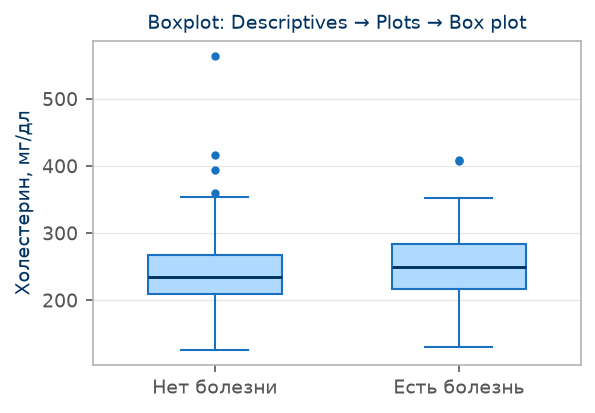
\includegraphics[width=\linewidth]{plot_boxplot.png}
    \column{0.32\linewidth}
      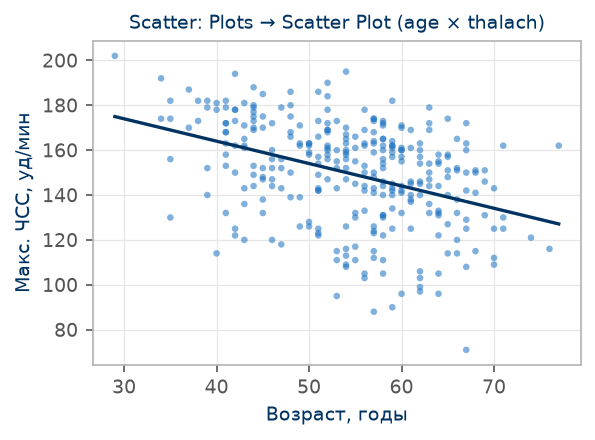
\includegraphics[width=\linewidth]{plot_scatter.png}
    \column{0.32\linewidth}
      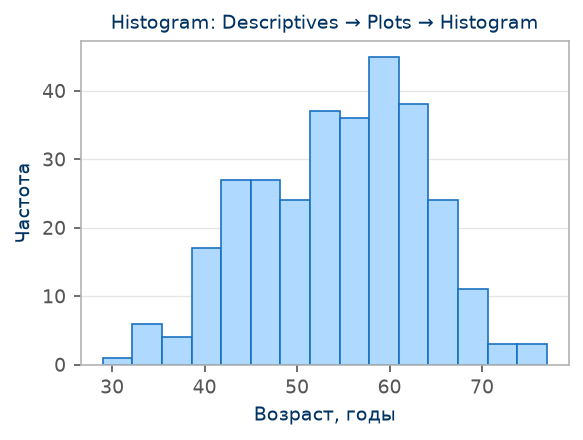
\includegraphics[width=\linewidth]{plot_histogram.png}
  \end{columns}
  \begin{block}{Подписи обязательны}
    Ось $X$, ось $Y$, заголовок, единицы измерения. График без подписей --- картинка, а не результат. В Jamovi: \texttt{Plot \& Axis Titles}.
  \end{block}
  \begin{alertblock}{Задание (3 минуты)}
    Scatter \texttt{age} $\times$ \texttt{oldpeak}, подписать оси, добавить линию тренда.
  \end{alertblock}
\end{frame}

\section{ИИ}

\begin{frame}{ИИ в анализе данных: рамки}
  \small
  \begin{columns}[T,onlytextwidth]
    \column{0.48\linewidth}
      \begin{block}{ИИ --- калькулятор, не врач}
        \begin{itemize}
          \item Помогает объяснить таблицу, набросать тест, шаблон статьи
          \item Не отвечает за интерпретацию; решение --- за исследователем
        \end{itemize}
      \end{block}
    \column{0.48\linewidth}
      \begin{block}{Два главных риска}
        \begin{itemize}
          \item \textbf{PHI:} данные пациентов в чат --- этическое и правовое нарушение
          \item \textbf{Галлюцинации:} ИИ уверенно выдаёт несуществующие функции
        \end{itemize}
      \end{block}
  \end{columns}
  \begin{block}{Правило проверки}
    Код или метод от ИИ --- сначала на учебном наборе, потом сверка с документацией.
  \end{block}
  \begin{block}{Честно про Jamovi}
    Официального ИИ-помощника в классическом Jamovi нет; сторонние модули сегодня не показываем.
  \end{block}
\end{frame}

\section{Итоги}

\begin{frame}{Три главных вывода}
  \begin{enumerate}
    \item \textbf{Jamovi закрывает базовый анализ без кода}: импорт --- описание --- тесты --- графики, всё меню.
    \item \textbf{$p$-value и CI читаются одинаково везде}: меняется таблица, принцип --- тот же.
    \item \textbf{Выбор критерия} --- это три вопроса: тип данных, тип групп, нормальность.
  \end{enumerate}
  \begin{block}{Что дальше}
    \begin{itemize}
      \item Датасет, презентация и запись --- в репозитории заседания
      \item Возможные продолжения: расширения Jamovi, разбор собственного исследования
      \item Вопросы --- сейчас
    \end{itemize}
  \end{block}
\end{frame}

\begin{frame}{Литература и источники}
  \small
  \begin{columns}[T,onlytextwidth]
    \column{0.5\linewidth}
      \textbf{Книги}
      \begin{itemize}
        \item Vu J., Harrington D. Introductory Statistics for the Life and Biomedical Sciences. --- OpenIntro, 2021. Свободно: openintro.org/book/biostat
        \item Петри А., Сэбин К. Наглядная медицинская статистика. --- М.: ГЭОТАР-Медиа, 2021
        \item van Belle G. и др. Biostatistics: A Methodology for the Health Sciences. 2nd ed. --- Wiley, 2008
        \item Гланц С. Медико-биологическая статистика. --- М.: Практика, 1999
      \end{itemize}
    \column{0.5\linewidth}
      \textbf{Источники}
      \begin{itemize}
        \item Документация jamovi --- docs.jamovi.org
        \item Датасет UCI Heart Disease (Detrano et al., 1989) --- archive.ics.uci.edu
        \item Wasserstein R., Lazar N. The ASA Statement on p-Values. --- The American Statistician, 2016
        \item BMJ «Statistics notes» (Bland \& Altman) --- заметки по темам заседания
      \end{itemize}
  \end{columns}
\end{frame}

\workshopcontacts

\end{document}
